\chapter{Design}
\label{Chapter:Design}
With a clear identification of the problem, sufficient motivations, and well defined requirements, based on informed research a design incorporating all the details could be developed. Although the design process is being carried out before the implementation phase, it is important to note that these are only initial designs. Due to the agile methodology the design and implementation processes are essentially interleaved with one another. This allows for design of one component to be completed, which can then be implemented and improved by feedback. The design of the next component will be influenced by the feedback and lessons learnt from the development of the previous components.

The first part of the design process involved coming up with an overall system architecture, which is discussed in section 5.1. However the first component to be designed would be the database as this is required by almost all other components in the system and should be readily available. In order to develop the database, a level of data collection was also necessary which is briefly touched on throughout this section.

The remainder of the design section covers the user interface design in depth for each of the significant pages on the system. The consistency of the user interface as well as design choices such as colours and layouts are also discussed. Finally a brief overview of responsive mobile design is provided.

\section{System Design and Architecture}
The systems' overall layered design and architecture can be seen in figures \ref{fig:LayerArchitecture} and \ref{fig:SystemArchitecture} respectively. The former provides a high-level overview of all the components in the system and the interaction between these components using various technologies. The latter, however, provides an in-depth view of the data flow and the processes in the system.

\subsection{High Level Design}
The diagram in figure \ref{fig:LayerArchitecture} shows a high-level overview of the system design. There are three main layers of the system which make up the web application. These are the:

\begin{itemize}
\item User Interface (UI) layer, developed using HTML 5 and CSS3
\item Application Services (AS) layer, responsible for performing the majority of system logic in PHP
\item Database Management System (DBMS) layer, which allows the storage and retrieval of data using MySQL
\end{itemize}

On its own, the AS layer would be insufficient to provide users with tailored content as PHP is not powerful enough to process large data quantities. For this reason, an additional `background' layer is added to the system. This layer is broken down into data collection and data analysis and will be responsible for running analysis algorithms as scheduled jobs that will analyse the data and update the database. The inclusion of this additional layer increases the efficacy of data processing, meaning the AS layer only needs to output already processed data.

\begin{figure}[H]
  \centering
  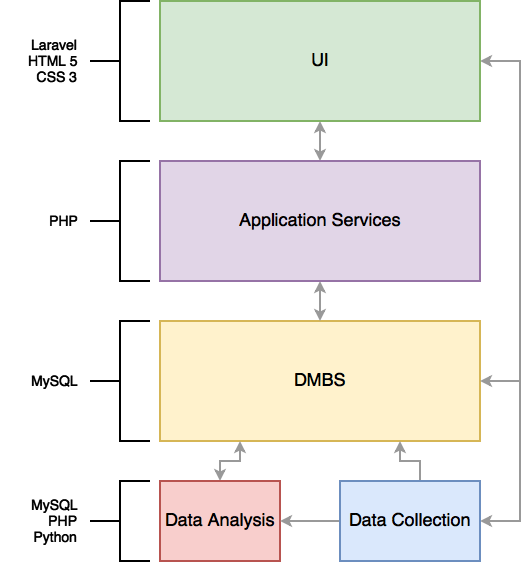
\includegraphics[width=0.5\textwidth]{Images/Design/LayerArchitecture}
  \caption{High-Level System Design} \label{fig:LayerArchitecture} 
\end{figure}

\subsection{Overall System Architecture}
The operation of the system is broken down into five stages: 

\begin{itemize}
\item Data collection
\item Data processing
\item Recommendation
\item Content filtering 
\item User interface
\end{itemize}

The functionality of each of these stages is implemented in multiple layers of the high-level system design in figure \ref{fig:LayerArchitecture}. The data collection stage will primarily be responsible for collecting data about the user, such as their personal information, as well as capturing the content, text or photos, posted by the user and storing this in the database so that it may be processed and visualised later. This raw data is represented by the black lines with arrows indicating the direction of the data flow. Additionally, the data collection process will also collect data such as tags, categories and possibly tweets from Twitter and store this so that it may be used for training machine learning models. This stage can be extended to collect data from other sources such as news feeds for better categorisation and trend plotting. The stored posts then undergo processing to assign tags explicitly used by the author, and at the same time also assign tags detected by the algorithm based on the content of the post. Once the post has been tagged, the post is assigned to a category based on its tags. The processed data, represented by green lines, is then stored in the database with state fields which indicate that the tuples have been processed. Once the data has been converted to a standard format and has been correctly associated, based on the viewers' settings, the appropriate recommendation algorithm is executed, which outputs recommended posts and users for each user. The recommended data, represented by red lines, is now held in separate data storage so that it can quickly be fetched by the server and presented to the user. However, before we can present this data to the user, we need to filter it as it may contain abusive content. This process is carried out by the content filtering stage which looks at the abuse score assigned to each post and filters out abusive posts. The abuse score is computed by a logistic regression model, in the data analysis stage in figure \ref{fig:LayerArchitecture}, trained on content from Twitter collected in the data collection stage. The original posts storage is updated at regular intervals by a scheduled job. Finally, the filtered content, represented by blue lines, can be displayed to the user on various pages and widgets throughout the site. 

\begin{figure}[H]
  \centering
  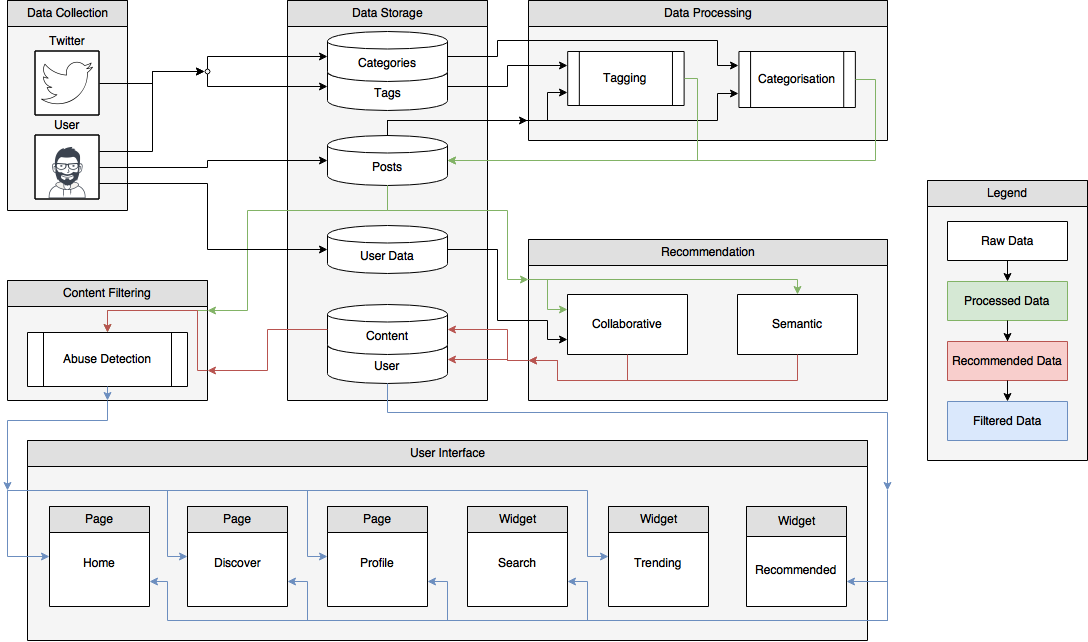
\includegraphics[width=1.0\textwidth]{Images/Design/SystemArchitecture}
  \caption{Proposed System Architecture Diagram} \label{fig:SystemArchitecture} 
\end{figure}
\section{Data Collection}
Fidelis relies heavily on data collected from the users and external sources so that it can successfully provide meaningful content to its users. Because there will be no user data upon launch of the social network, data will need to be collected beforehand so that the functionality is apparent immediately, thus making Fidelis an attractive platform for users to register to. Once users start using Fidelis, data will then need to be continually collected so that the system is able to learn about the users and recommend to them relevant content. In particular, training sets must be collected for the machine learning models used to detect abuse and categorise content and user data must be collected to authenticate access to the site. In addition, when testing the site, template data is used to populate the site to ensure that data is correctly fetched from the database and then displayed. This section discusses the methods which will be used to collect the data so that it can be used in the social network.

\subsection{Training Data}
Both abuse detection and tag categorisation use supervised machine learning techniques in order to classify posts.  Therefore, data must be collected with which the machine learning models can be trained. Because the data will be immutable, storing the training data in Comma-Separated Values (CSV) files will be sufficient.

As part of their competition `Detecting Insults in Social Commentary', Kaggle provided CSV datasets containing sample messages alongside a boolean attribute, representing whether that post is determined to be abusive or not ~\cite{Kaggle:Dataset}. This data is publicly available and the messages are in the same format as Fidelis posts would be expected to be, making it suitable for use when training the model.

Whereas Kaggle have curated a clean dataset which can be readily used in training the abuse detection, a dataset containing sample posts alongside their category was not available. However, Zubiaga and Ji have published a dataset containing Tweet IDs with their corresponding topic tag ~\cite{Zubiaga:Tweets}. For this dataset to be usable in this project when predicting the category of posts on the social network, further data must be collected from the Twitter API so that the text of the Tweet can be determined, since it is the text which contains the features from which the model can learn.

\subsection{Template Data}
Template data is required during implementation of the social network in order to be able to model how data fetched from the database will be reflected throughout the site. Although some of the data will not be used when the site goes live, it is important that the template data closely resembles the format the data is expected to be in when the database is populated with the real data, so that any possible issues with regards to data being collected and displayed can be identified effectively.

Each of the comments, followers, posts, users and votes tables are populated with template data which will be used for testing the site and removed when the site goes live. In addition to this, further template data can be provided in the categories, category\_tag, quotes, tags and wallpapers tables. These tables will remain populated with the data, since the data stored in the tables provide functionality required on the launch of the site. For example, categories is used to store the default categories which are displayed on the Discover page, whereas the quotes and wallpapers tables store the quotes and images displayed on the home page of the site when the user is not logged in.

To ensure that the template data is authentic, the comments and posts are obtained either from existing social networks such as Facebook and Twitter or they will be suggested by would-be users of Fidelis. In addition, these would-be users can be added as template users to the site.

\subsection{User Authentication}
Data will need to be collected about the user in order to authenticate access to private areas within the site. In Fidelis, this will use a form which is filled in by the user during registration, which includes password fields which will grant the user access to the site in the future. This password will then be encrypted and stored in the users table. The user's email address will also be collected and stored so that the password can be recovered in the case that the user forgets their password. This is consistent with the methods used to collect authentication data in current social networks.
\section{Data Processing}
Processing data in Fidelis plays a key role in meeting the requirements set by the stakeholders. Data processing will occur through abuse detection on posts to remove abusive and derogatory content from the site, content filtering to recognise trending topics and automatically categorise user-submitted posts, recommendations to provide users with fresh content to engage with, and finally reputation scoring to allow users to quantify content and user trustworthiness.

\subsection{Abuse Detection}
\label{sec:abuse-detection}
Abuse detection will be performed on Fidelis to filter out derogatory and abusive content from the users post feed. Performing abuse detection will provide users with confidence that they will not encounter content they deem offensive whilst on Fidelis. Different users will have varying levels of tolerance towards abuse, so users should be allowed to determine what abuse is filtered from their feed. To this end, users should be able toggle their `tolerance' level, which will determine what content is removed or included on their feed. Allowing toggling of abuse level means that we are not interested in a binary classification problem, and instead move towards the idea of how likely a user will find a piece of text offensive. Whereas with the original approach we had either 0 (post is not abusive) or 1 (post is abusive), introducing a probabilistic score will enable the user to select their own tolerance level. The following sections will look at the various stages that need to be considered for abuse detection. Namely, data pre-processing, model building and data handling

\subsubsection{Data Pre-Processing}
As mentioned in Chapter \ref{Chapter:Research}, abuse detection is regularly achieved by building a classifier trained on features extracted from relevant texts. Before a classifier can be trained, the data must first be fetched and cleaned. Cleaning data is important before processing as `dirty' data can have an adverse effect on model performance. In the case of natural lanuage processing, data cleaning can involve \cite{han2011data}:
\begin{itemize}
\item Removing stop words such as ``the'' or ``a'', 
\item Removing punctuation, although it should be noted that certain punctuation should be kept with the original text, especially when performing sentiment analysis
\item Converting text to be all lower or upper-case
\item Removing HTML mark-up
\item Removing apostrophes
\end{itemize}

When building a model for text classification, the model is trained on significant features extracted from the text. These features are elements from the text, and common techniques used when extracting features during natural language processing are discussed in Chapter \ref{Chapter:Research}. As part of pre-processing, features must first be extracted from the data before the model is trained.

\subsubsection{Model Building}
Abuse detection is a classification problem; a piece of text is either abusive or not. A variety of machine learning classifiers can be used for this, but for our purposes the Support Vector Machine (SVM) and Logistic Regression (LR) models will be used. SVMs have been shown to be one of the best performing models for text classification \cite{joachims1998text}. This has also been shown for LR models \cite{genkin2007large}, with performance for these models being shown to be ``at least as effective as those produced by support vector machine classifiers''. Models will be built by training them on the set of features extracted from the data. To ensure that the produced classifier does not overfit the training data, and instead generalises well to the plethora of unseen data it will receive in the form of user posts cross-validation will be used. Cross-validation is a training technique that serves this purpose, and splits a dataset into separate training and testing sets \cite{scikit:cross-val}. Model performance is dependent on features extracted from data, and additionally on the parameters chosen for the model, which in turn are dependent on the data itself. To maximise model performance, parameters must be tuned to assess their suitability for the model and given data. Algorithm \ref{alg:abuse} provides a very high-level overview of the process of building a model for text classification.

\begin{algorithm}
\caption{Algorithm for training model}
\label{alg:abuse}
\begin{algorithmic}[1]
\State $data\gets getTwitterData$
\State $train\gets getTrainingData(data)$
\State $test\gets getTestData(data)$
\State $cleanData\gets cleanData(data)$
\State $features\gets extractFeatures(data)$
\State $classifier\gets trainModel(features)$
\State Test $classifier$ using $test$
\State Save $classifier$
\end{algorithmic}
\end{algorithm}

\subsubsection{Handling Abusive Data}
On Facebook, 55 million status updates are made daily \cite{kissmetrics:fb-stats}. This equates to \textasciitilde 636 posts per second. It would therefore be infeasible to expect to categorise posts during real-time due to the sheer number of posts that can be encountered. To counteract this, the classifier should be run on posts daily at a chosen time. The results from classifying posts as abusive should not only be reflected in them being hidden from the users post feed - the reputation score of the abusive post and the user making the post should be updated accordingly. Algorithm \ref{alg:abuse-classification} shows the procedure that will be used to classify user posts made on Fidelis.

\begin{algorithm}
\caption{Algorithm for post classification}
\label{alg:abuse-classification}
\begin{algorithmic}[1]
\State $clf\gets loadClassifier$
\State $posts\gets getAllUserPosts$
\For{$post$ in $posts$}
	\State Classify $post$ using $clf$
	\If{$post$ is abusive}
		\State $author\gets getPostAuthor(post)$
		\State Update reputation score for $post$ and $author$
	\EndIf
\EndFor
\end{algorithmic}
\end{algorithm}

The classifier built for abuse detection will not be perfect, and there is a chance that it will not be able to detect all types of abusive content posted to Fidelis. The classifier must therefore be re-trained with posts that are manually flagged by users as offensive. Using this new data, the accuracy of the classifier can improve over time. Algorithm \ref{alg:model-improvement} shows how posts that are flagged as abusive by the user will be retrieved and used to re-train the classifier.

\begin{algorithm}
\caption{Algorithm for re-training the classifier}
\label{alg:model-improvement}
\begin{algorithmic}[1]
\State $clf\gets loadClassifier$
\State $reports\gets getReportedPosts$
\State $cleanReports\gets cleanData(reports)$
\State $reportFeatures\gets extractFeatures(cleanReports)$
\State Re-train $clf$ using $reportFeatures$
\end{algorithmic}
\end{algorithm}
\subsection{Content Filtering}
The filtering of content allows the users to receive tailored content, which is more likely to be of interest of them and therefore instils trust in the social network. To maximise the performance of content filtering and increase the chances of overall project success, three different models are considered: Na\"ive Bayes, SVMs and Stochastic Gradient Descent (SGD). Once the models are able to successfully detect the category of a post, the post category can be updated in the database, which will allow filtered feeds to retrieve the relevant content to be displayed to the user. 

This section will discuss the design decisions made for the content filtering throughout each stage of the process. This includes the preprocessing of the data and the training of the model as well as algorithms for testing the efficacy of the model and using it to predict new posts as they are made on Fidelis. There are similarities between the processing performed in this section and section \ref{sec:abuse-detection} due to similarities in NLP techniques discussed, however there are significant differences in how the features are extracted and how the models are built.

\subsubsection{Data Preprocessing}
Before being able to train the model, preprocessing must be carried out on the data. This is made up of two parts: data cleaning and feature extraction. Algorithm \ref{alg:content-filter-cleaning} shows how data cleaning is performed, which removes any non-ASCII characters, Twitter entities (such as mentions and URLs), stop words and punctuation as these objects aare not informative of the topic of the post. Pre-processing also lemmatizes the words so that words with the same stem become the identical. If the overall number of characters in the cleaned post is less than 20, the empty set is returned instead of the cleaned post, because it is deemed to not be informative enough to be used in the training sample.

\begin{algorithm}[H]
\caption{Content filter cleaning algorithm}
\label{alg:content-filter-cleaning}
\begin{algorithmic}[1]
\Function{clean}{$post$}
	\State $clean\gets \emptyset$
	\State $post\gets post - nonAsciiChars(post) - cleanTwitterEntities(post)- removePunc(post)$
	\ForAll{$word \in post$}
		\State $word\gets lemmatize(word)$
		\If{Word $word \in stopwords$} 
			\State \textbf{break} 
		\EndIf
		\If{$len(word) < 3$} 
			\State \textbf{break} 
		\EndIf
		\State Add $word$ to $clean$
	\EndFor
	\If{$numChars(clean) < 20$}
		\State \Return{$\emptyset$}
	\Else
		\State \Return{$clean$}
	\EndIf
\EndFunction
\end{algorithmic}
\end{algorithm}

After cleaning the data, features need to be extracted from the cleaned posts, which act as attributes that the machine learning model can learn from. The algorithm for this stage is shown in algorithm \ref{alg:content-filter-features}, which takes the data frame consisting of cleaned post-category pairs in the training set as input ($dataset$) and outputs the new dataframe $tf\_idf$, which contains the term frequency-inverse document frequency (TF-IDF) score of each uni- and bigram in the cleaned posts. Bigrams are used because two consecutive words within a cleaned post may be more representative of a topic than a single word in isolation. The functions $countVectorize()$ takes the data frame containing ngrams and converts it such that each ngram is an attribute and the value of that attribute for each post is the number of times that particular ngram appears in the post. $tfidfTransform()$ then takes this data frame and replaces the counts with the TF-IDF score.

\begin{algorithm}[H]
\caption{Content filter feature extraction}
\label{alg:content-filter-features}
\begin{algorithmic}[1]
\Function{featureExtraction}{$dataset$}
\State $tf\_idf\gets \emptyset$
\ForAll{Row $row \in dataset$}
	\State $row[clean\_post]\gets row[clean\_post]\cup getBigrams(row[clean\_post])$
\EndFor
\State $tf\_idf\gets countVectorize(dataset)$
\State \Return{$tfidfTransform(tf\_idf)$}
\EndFunction
\end{algorithmic}
\end{algorithm}

\subsubsection{Model Building}
Independent of the type of model chosen for implementation, the pipeline in algorithm \ref{alg:content-filter-pipeline} demonstrates how the model is built. In the case where the model is being built for the Fidelis site, the entire training set is used initially, because no content exists on the site. However, the model can be retrained on newer posts when enough user-created content is available.

\begin{algorithm}[H]
\caption{Content filter model pipeline}
\label{alg:content-filter-pipeline}
\begin{algorithmic}[1]
\State $data\gets getDataset()$
\ForAll{Post $data[post]$}
	\State $data[post]\gets clean(data[post])$
\EndFor
\State $data\gets FeatureExtraction(data)$
\State $model \gets train(data)$
\end{algorithmic}
\end{algorithm}

Although algorithm \ref{alg:content-filter-pipeline} is sufficient for building a model for topic prediction, the algorithm needs to be adapted slightly so that the different models can be compared. This updated algorithm incorporates cross-validation. The algorithm used for building the models so that they can be evaluated is shown in algorithm \ref{alg:content-filter-cv}. The algorithm uses 10-fold cross-validation and then computes a score for the model based on the mean fraction of samples in the test set which is correctly predicted across each of the folds. The $randomSubsample()$ function splits the data into $n$ random sub-samples, creating an array of test sets. The algorithm can then be repeated for each of the techniques and the scores can be compared.

\begin{algorithm}
\caption{Content filter model cross-validation}
\label{alg:content-filter-cv}
\begin{algorithmic}[1]
\State $data\gets getDataset()$
\ForAll{Post $data[post]$}
	\State $data[post]\gets clean(data[post])$
\EndFor
\State $data\gets featureExtraction(data)$
\State $testsets\gets randomSubsample(data, 10)$
\State $score\gets 0$
\ForAll{$test \in testsets$}
	\State $training\gets data\setminus test$
	\State $model\gets train(data)$
	\State $score\gets score + model.predict(test).score$
\EndFor
\State $score\gets score/10$
\end{algorithmic}
\end{algorithm}

\subsubsection{Predicting Topics}
Once the model is built, it can then be deployed to predict the categories of tags. The tags themselves act as sub-categories to the main categories which are displayed on the sidebar on the discover page. For example the tag \textit{\#watfordfc} should be categorised under sport and therefore the posts containing that tag would be displayed in the sport section on the discover page. The algorithm in algorithm \ref{alg:content-filter-predict} should run at regular intervals to predict the categories of recently made tags and add them to the category-tag table. Although the model is trained on entire posts, taqs are sufficiently informative to categorise them.

\begin{algorithm}
\caption{Content filter tag prediction}
\label{alg:content-filter-predict}
\begin{algorithmic}[1]
\Function{predict}{Model $model$, Tags $tags$}
	\State $tags\gets uncategorised(tags)$
	\State $topics\gets model.predict(tags)$
	\State $tags \gets tags.addColumn(topics)$
	\ForAll{Row $tag \in tags$}
		\State Add $(Row[tag],Row[topic])$ to Category-Tag table
	\EndFor
\EndFunction
\end{algorithmic}
\end{algorithm}

Furthermore, the post itself is categorised, so that posts without tags can be assigned to a category on the discover page. Algorithm \ref{alg:post-predict} shows how the post-tag table is updated to include the post category as assigned to it by the model prediction. Moreover, it allows the user to update the topic of the post in case the post is incorrectly categorised or if the post should not belong to any category. These post categorisations can then be used to train the model in the future so that the model is kept up-to-date. Depending on how quickly the model is able to categorise a post, the user may be prompted to change the category. If the prediction is quick, the user can be prompted to confirm the chosen category is correct, which will help ensure the model is trained on reliable data in the future. However, if the prediction is slow, the user can not wait to be prompted to confirm the category of the post. For the data to all be assigned a correct category, the user would have to change the category without prompt, which could affect the integrity of the data when training future models.   

\begin{algorithm}
\caption{Content filter post prediction and update}
\label{alg:post-predict}
\begin{algorithmic}[1]
\Function{predict}{Model $model$, Post $post$}
	\State $topic\gets model.predict(post)$
	\State Add $(Row[tag],Row[topic])$ to Post-Tag table
	\If{$topic$ is changed by user}
		Delete original $topic$ from Post-Tag table
		Add new $topic$ to Post-Tag table
	\EndIf
\EndFunction
\end{algorithmic}
\end{algorithm}
\subsection{Content Recommendation}
\label{sec:ContentRecommendation}
Recommendations are a key component to Fidelis, and this section will look at the design of the algorithms for this purpose. Collaborative-based filtering was chosen as the filtering technique for recommendations. Justification for this is apparent in the technique itself; collaborative-filtering focuses on using the opinions of like-minded users, coupled with items rated by the user in the past. This sets up recommendations for success as they are much more likely to be greeted positively by the user. Given the nature of Fidelis as social network, resources in terms of previously rated items (through votes on posts) and like-minded users will be available in abundance to generate strong recommendations. It is important to provide the user with choice for how they would like to receive recommendations. To this end, the user will be provided with the option to choose how their recommendations should be provided. The following sections will look at the algorithm that will be used to generate recommendations for users, and will also discuss three different recommendation flavours that will be offered to the user, giving them final say on how their recommendations are generated. 

\subsubsection{User Recommendations}
\label{sec:user-recommendations}
Users are likely to interact with recommendations they receive on a daily basis. As such, algorithms generating recommendations should run on a daily basis. To generate recommendations, we must therefore first look at the number of recommendations already generated for each user. A user may choose not to interact with provided recommendations, so new recommendations should be made only when a user has approved or rejected their current recommendations. For each user, their item vector should be retrieved. The item vector will correspond to the features discussed in Chapter \ref{Chapter:Research}. The set of candidate recommendations for the user will be determined by what recommendation method they have chosen. Before checking for similarity between the user and the candidate recommendations, all users the user already follows, has blocked or has rejected as a recommendation should be removed from the candidate set. In the event that there are no candidate users, a default set of recommendations will be provided for the user. Using the retrieved collection of candidate recommendations, each user in this collection will be assessed to determine whether the similarity between them and the user is sufficiently large. Suitability between users will be determined using a threshold value. We are only interested in similarities that are at least as large as this value, as similarities less than the threshold value would mean that the two users in question are not similar. Only those users with a similarity greater than the threshold value should be provided as a recommendation. Similarity will be measured using cosine similarity. Cosine similarity is calculated using the following equation:
\begin{equation}
sim(\mathbf{A},\mathbf{B}) = \frac{\mathbf{A} \cdot \mathbf{B}}{\parallel\mathbf{A}\parallel \parallel\mathbf{B}\parallel} = = \frac{ \sum\limits_{i=1}^{n}{A_i  B_i} }{ \sqrt{\sum\limits_{i=1}^{n}{A_i^2}}  \sqrt{\sum\limits_{i=1}^{n}{B_i^2}} }
\label{eq:cos-similarity}
\end{equation}
Algorithm \ref{alg:user-recommendations} provides pseudocode for this process. Values for $similarityThreshold$ and $val$ should be set by the user.

\begin{algorithm}[H]
\caption{User recommendations algorithm}
\label{alg:user-recommendations}
\begin{algorithmic}[1]
\State $similarityThreshold\gets 0.7$
\State $val\gets 5$
\ForAll{users $u$}
	\State $method\gets getRecommendationMethod(u)$
	\State $currentRecommendations\gets getNumberOfRecommendations(u)$
	\If{$currentRecommendations < val$}
		\State $uVector\gets getItemVector(u)$
		\If{$method = Friend$-$of$-$a$-$Friend$}
			\State $users\gets getFOFUsers(u)$
		\EndIf
		\If{$method = Explorer$}
			\State $users\gets getExplorerUsers(u)$
		\EndIf
		\If{$method = Hybrid$}
			\State $fof\gets getFOFUsers(u)$
			\State $explorer\gets getExplorerUsers(u)$
			\State $users\gets fof \cap explorers$
		\EndIf
		
		\State $uFollowing\gets getFollowing(u)$
		\State $uBlocked\gets getBlockedUsers(u)$
		\State $uRejected\gets getRejectedRecommendations(u)$
		\State $users = users \setminus uFollowing \setminus uBlocked \setminus uRejected$
		
		\If{$\left\vert{users}\right\vert = 0$}
			\State $getDefaultUsers$
		\Else
			\For{$v$ in $users$}
				\State $vVector\gets getItemVector(v)$
				\State $similarity\gets measureSimilarity(uVector, vVector)$
			
				\If{$similarity \geq similarityThreshold$}
					\State $storeRecommendation(v)$
				\EndIf
			\EndFor
		\EndIf
	\EndIf
\EndFor
\end{algorithmic}
\end{algorithm}

We will now look at each of the possible user sets for candidate recommendations. In particular, we will observe a general overview of the method for user selection and involves ourselves with a discussion on the method itself with regards to the wider system.

\begin{figure}[h]
	\centering
	\begin{subfigure}[b]{.3\linewidth}
		
\includegraphics[height=1.7in]{Images/Design/facebook}
		\caption{}
		\label{fig:fof-facebook}
	\end{subfigure}
	\begin{subfigure}[b]{.5\linewidth}
		
\includegraphics[width=1\linewidth]{Images/Design/linkedin}
		\caption{}
		\label{fig:fof-linkedin}
	\end{subfigure}
	\caption{Friend-of-a-Friend recommendations from (a) Facebook and (b) Twitter}
	\label{fig:fof}
\end{figure}

\paragraph{Friend-of-a-Friend Users}
With this method, candidate recommendations for a user $A$ are all users $C$ where $A$ follows $B$ and $B$ follows $C$. This method uses like-minded users for recommendations, and exploits the transitive nature of the ``following'' relationship. It is a popular technique used by numerous social networks, including Facebook (Figure \ref{fig:fof-facebook}) and Linkedin (Figure \ref{fig:fof-linkedin}). This option will allow the user to generate ``safer'' recommendations by using the idea that ``if $A$ trusts $B$, and $B$ trusts $C$, $A$ will most likely also trust $C$''. This is not always the case, but mostly holds true. It is important to give users this choice as it provides them more control over who enters their trust circle. Although one of the project aims is to burst opinion bubbles through exposure to different and trusted views, users must still be provided with this option. The function in Algorithm \ref{alg:fof-users} provides a procedure for retrieving ``$C$'' users. 

\begin{algorithm}[H]
\caption{Function for getting Friend-of-a-Friend users}
\label{alg:fof-users}
\begin{algorithmic}[1]
\Function{getFOFUsers}{User u}
	\State $users = \emptyset$
	\State $uFollowing\gets getFollowing(u)$
	\For{$f$ in $uFollowing$}
		\State $fFollowing\gets getFollowing(f)$
		\State Add $fFollowing$ to $users$
	\EndFor
	\State \Return{$users$}		
\EndFunction
\end{algorithmic}
\end{algorithm}

\paragraph{Explorer Users}
Fidelis aims to expose users to opinions and users they may not initially interact with. Explorer users are chosen for exactly this reason. Candidate recommendations are found by finding users' favourite tags to post in and looking at other users who post in the same tag. This user collection method combines the users rated items and looks at like-minded users. By deviating from the users trust circle, we are more likely to generate recommendations that will broaden user opinions by finding other users who care about the same topics, but will naturally hold different views on them. This method seeks to expand a users trust circle beyond current opinions held by them. The function in Algorithm \ref{alg:explorer-users} shows the procedure for collecting Explorer users. $N$ is used to determine the number of tags that will be searched for candidate recommendations. The function in Algorithm \ref{alg:explorer-users} shows this procedure.

\begin{algorithm}[H]
\caption{Function for getting Explorer users}
\label{alg:explorer-users}
\begin{algorithmic}[1]
\Function{getExplorerUsers}{User u}
	\State $threshold\gets 75$
	\State $users\gets \emptyset$
	\State Get $N$ top tags $u$ posts in
	\For{$tag t = 1$ to $N$}
		\State Get all users $v$ posting in $t$
		\If{$reputationOf(v) >= threshold$}
			\State Add $v$ to $users$
		\EndIf
	\EndFor
	\State \Return{$users$}
\EndFunction
\end{algorithmic}
\end{algorithm}

\paragraph{Hybrid Users}
Using this method aims to find the middle ground between the two aforementioned techniques. The intersection between Explorer and Friend-of-a-Friend users, as shown in Figure \ref{fig:hybrid}, is returned as the set of candidate recommendations. 

\begin{figure}
\centering
\begin{tikzpicture}[
    thick]
    \draw [fill=cyan, fill opacity=0.5, name path=c1] (0,0) circle (2cm);
    \draw [fill=orange, fill opacity=0.5, name path=c2] (3,-1) circle (2.5cm);
    \draw (0,0) ++(120:2cm) -- ++(120:2.2cm) node [fill=white,inner sep=5pt](a){Friend-of-a-Friend};
    \draw (3, -1) ++(30:2.5cm) -- ++(30:2.6cm) node [fill=white,inner sep=5pt](b){Explorer};
    \path [name intersections={of=c1 and c2,by=cs}];
    \draw (cs) -- ++(.5,1) node [fill=white,inner sep=5pt](c){Hybrid};
\end{tikzpicture}
\caption{Hybrid user selection}
\label{fig:hybrid}
\end{figure}

\paragraph{Default Recommendations}
If all aforementioned methods fail to return a set of candidate recommendations, the system should revert to default candidate recommendations. This method will return either the $N$ most popular or reputable users on Fidelis. The function in Algorithm \ref{alg:default-users} shows this procedure for most popular users, but the same procedure can be re-used for getting the most reputable users.

\begin{algorithm}[H]
\caption{Function for getting default users}
\label{alg:default-users}
\begin{algorithmic}[1]
\Function{getDefaultUsers}{User u}
	\State $users\gets \emptyset$
	\State $users\gets getMostPopularUsers$
	\State $users\gets sortDescending(users)$
	\State \Return{$N$ top users from $users$}
\EndFunction
\end{algorithmic}
\end{algorithm}

\subsubsection{Post Recommendations}
\label{sec:post-recommendations}
Similarly to user recommendations, users will interact with content recommendations made for them daily and so new post recommendations should be generated for them daily also. Again, before any new recommendations are made we must look at how many recommendations the user currently has. By doing this, we limit any unnecessary computation. In the case of content recommendations, user item vectors will not be used. It was instead decided to use the reputation of a given post, rather than the similarity between the user recommendations are being generated for and the author of the post. The justification behind this is that user recommendations should focus on locating like-minded users, whereas content recommendations should avoid this to diversify the content made available to users. Providing recommendations in this manner again emphasises the desire for Fidelis to break the constraints of the ``echo chamber effect'' currently restricting most social media platforms. By letting the user pick a reputation threshold for recommendations generated for them, we can ensure that users trust their recommendations and can confidently interact with them knowing they are trustworthy. Algorithm \ref{alg:post-recommendations} provides the pseudocode for the procedure described above. 

\begin{algorithm}[H]
\caption{Post recommendations algorithm}
\label{alg:post-recommendations}
\begin{algorithmic}[1]
\State $val\gets 5$
\State $reputationThreshold\gets 0.7$
\ForAll{users $u$}
	\State $method\gets getRecommendationMethod(u)$
	\State $currentRecommendations\gets getNumberOfRecommendations(u)$
	\If{$currentRecommendations < val$}
		\If{$method = Friend$-$of$-$a$-$Friend$}
			\State $posts\gets getFOFPosts(u)$
		\EndIf
		\If{$method = Explorer$}
			\State $posts\gets getExplorerPosts(u)$
		\EndIf
		\If{$method = Hybrid$}
			\State $fof\gets getFOFPosts(u)$
			\State $explorer\gets getExplorerPosts(u)$
			\State $posts\gets fof \cap explorers$
		\EndIf
		
		\State $uVoted\gets getVotedPosts(u)$
		\State $uBlocked\gets getBlockedPosts(u)$
		\State $posts = posts \setminus uVoted \setminus uBlocked$
		
		\If{$\left\vert{posts}\right\vert = 0$}
			\State $getDefaultPosts$
		\Else
			\For{$p$ in $posts$}
				\If{$getReputation(p) \geq reputationThreshold$}
					\State $storeRecommendation(p)$
				\EndIf
			\EndFor
		\EndIf
	\EndIf
\EndFor
\end{algorithmic}
\end{algorithm}

We will again look at how each of the four recommendation techniques will generate candidate post sets. By providing the user with different ways recommendations can be generated for them will again ensure that users are in control of content they will interact with. 

\paragraph{Friend-of-a-Friend posts} Candidate recommendations using this method will build on the follows relationship mentioned earlier in Chapter \ref{sec:user-recommendations} by retrieving the posts from Friend-of-a-Friend users. Getting content in this manner will provide users with a selection of posts that are likely to agree with their own sentiments. 

\begin{algorithm}[H]
\caption{Function for getting Friend-of-a-Friend posts}
\label{alg:fof-content}
\begin{algorithmic}[1]
\Function{getFOFUsers}{User u}
	\State $posts\gets \emptyset$
	\State $uFollowing\gets getFollowing(u)$
	\For{$f$ in $uFollowing$}
		\State $fFollowing\gets getFollowing(f)$
		\For{$g$ in $fFollowing$}
			\State $gPosts\gets getPosts(g)$
			\State Add $gPosts$ to $posts$
		\EndFor  
	\EndFor
	\State \Return{$posts$}		
\EndFunction
\end{algorithmic}
\end{algorithm}

\paragraph{Explorer posts} Explorer post recommendations stress the idea previously mentioned about removing the constraints of the ``echo chamber effect''. By considering other users who post in the same categories as the user recommendations are being generated for, we only consider posts that the user will be interested in. Without considering the similarity between the authors of these posts and the user themselves, we increase the likelihood of exposing users to content they would not normally interact with.

\begin{algorithm}[H]
\caption{Function for getting Explorer posts}
\label{alg:explorer-content}
\begin{algorithmic}[1]
\Function{getExplorerPosts}{User u}
	\State $posts\gets \emptyset$
	\State $users\gets getExplorerUsers(u)$
	\For{$u$ in $users$}
		\State $uPosts\gets getPosts(u)$
		\State Add $uPosts$ to $posts$
	\EndFor
	\State \Return{$posts$}
\EndFunction
\end{algorithmic}
\end{algorithm}

\paragraph{Hybrid posts} Using this method aims to find the middle ground between the two aforementioned techniques. We take a similar approach as to before and return the intersection between Explorer and Friend-of-a-Friend posts as the set of candidate recommendations.

\paragraph{Default posts} Default post recommendations will return the $N$ most popular or reputable posts made on Fidelis. . The function in Algorithm \ref{alg:default-posts} shows the procedure for retrieving the most popular posts, but the same procedure can be re-used for getting the most reputable posts.

\begin{algorithm}[H]
\caption{Function for getting default posts}
\label{alg:default-posts}
\begin{algorithmic}[1]
\Function{getDefaultPosts}{}
	\State $posts\gets \emptyset$
	\State $posts\gets getMostPopularPosts$
	\State $posts\gets sortDescending(posts)$
	\State \Return{$N$ top posts from $posts$}
\EndFunction
\end{algorithmic}
\end{algorithm}
\subsection{Reputation Scoring}
It seems clear that collaboration events are a popular method of assessing reputation in online systems. The Sporas and Histos algorithms demonstrate mechanisms for this scoring using collaboration events \cite{mcnally2013} \cite{zacharia2000}. Ultimately, however, these algorithms did not meet the requirements for reputation scoring in this case. The Fidelis system would in theory serve a very large, complex network of users, which constrains the choice of reputation scoring algorithms. The proposed algorithm would need to run on the entire network each day (to score the reputation of both users and posts). Histos and Sporas would both be costly to run given the data stored in our database, therefore a similar, less complex method that adopts elements from Histos and Sporas was considered. This method involves simply performing a sum of each collaboration event, where each event type has a different weighting denoting the relative `importance' of the event in calculating reputation. The weighting functions are shown here for users and posts respectively

\begin{equation}
	\label{eq:rep_weight_user}
		w(c_u) = \left\{\begin{matrix}
			0.3 & if\ c\ is\ an\ upvote\ on\ a\ post\ by\ u\\ 
			-0.3 & if\ c\ is\ a\ downvote\ on\ a\ post\ by\ u \\ 
			0.1 & if\ c\ is\ an\ upvote\ on\ a\ comment\ by\ u \\ 
			-0.1 & if\ c\ is\ a\ downvote\ on\ a\ comment\ by\ u \\ 
			0.2 & if\ c\ is\ a\ comment\ on\ a\ post\ by\ u\\ 
			0.5 & if\ c\ is\ another\ user\ following\ u
		\end{matrix}\right.
\end{equation}
		
\begin{equation}
	\label{eq:rep_weight_post}
	 w(c_p) = \left\{\begin{matrix}
			0.1 & if\ c\ is\ an\ upvote\ on\ post\ p \\ 
			-0.1 & if\ c\ is\ a\ downvote\ on\ post\ p \\ 
			0.2 & if\ c\ is\ a\ comment\ on\ post\ p
	\end{matrix}\right.
\end{equation}

\noindent
where the weighting function \(w\) gives the weighting of a given collaboration event \(c\). The values of this function could, of course, be changed at any time in an attempt to produce more accurate reputation scoring. Once a reputation score has been calculated for each user, these scores will be normalised between 0 and 1. The pseudocode for this process is shown in algorithms \ref{alg:user-reputation} \ref{alg:post-reputation} for reputation scoring users and posts respectively.

\newcommand{\myindent}[1]{
\newline\makebox[#1cm]{}
}

\begin{algorithm}[H]
\caption{User reputation scoring algorithm}
\label{alg:user-reputation}
\begin{algorithmic}[1]
\State $users\gets getAllUsers()$
\ForAll{users $u$}
	\State $post\_upvotes\gets w(post\_upvote)\cdot getPostUpvotes(u)$
	\State $post\_downvotes\gets w(post\_downvote)\cdot getPostDownvotes(u)$
	\State $comment\_upvotes\gets w(comment\_upvote)\cdot getCommentUpvotes(u)$
	\State $comment\_downvotes\gets w(comment\_downvote)\cdot getCommentDownvotes(u)$
	\State $comments\gets w(comment)\cdot commentsgetPostComments(u)$
	\State $followers\gets w(follower)\cdot getFollowers(u)$
	\State $reputation\gets post\_upvotes + post\_downvotes + comment\_upvotes + comment\_downvotes \myindent{2.6} + followers$
\EndFor
\State $users\gets scaleReputation(users)$
\end{algorithmic}
\end{algorithm}

\begin{algorithm}[H]
\caption{Post reputation scoring algorithm}
\label{alg:post-reputation}
\begin{algorithmic}[1]
\State $posts\gets getAllPosts()$
\ForAll{posts $p$}
	\State $upvotes\gets w(upvotes)\cdot getPostUpvotes(p)$
	\State $downvotes\gets w(downvotes)\cdot getPostDownvotes(p)$
	\State $comments\gets w(comments)\cdot getPostComments(p)$
	\State $reputation\gets upvotes + downvotes + comments$
\EndFor
\State $posts\gets scaleReputation(posts)$
\end{algorithmic}
\end{algorithm}



\section{Database}
\section{Usability Principles}
Much progress has been made in the design of applications, making it more enjoyable for users to interact with a site and therefore increasing the likelihood of them recommending and revisiting the site. David Benyon composed usability principles which act as a guideline when designing applications with the user in mind \cite{Benyon}. These principles aim to improve consistency, familiarity and intuitiveness of applications.

The screenshots in figure \ref{fig:Twitter_Changes} highlight how the design of websites have changed. In particular, the design in image \ref{fig:Twitter_2017} shows how Twitter now use a more simplistic flat design, which uses bright colours so key areas of the page are clearly visible and separated. This is as opposed to the design in \ref{fig:Twitter_2006}, which uses a lot of gradients. This draws attention away from the important features on the site and makes it appear more cluttered. This shows how the designs have been adapted in order to make them more usable. Fidelis will also aim to make the application more usable through the use of design principles, as discussed in this section.

\begin{figure}[H]
	\centering
	\begin{subfigure}[t]{0.45\textwidth}
		\centering
		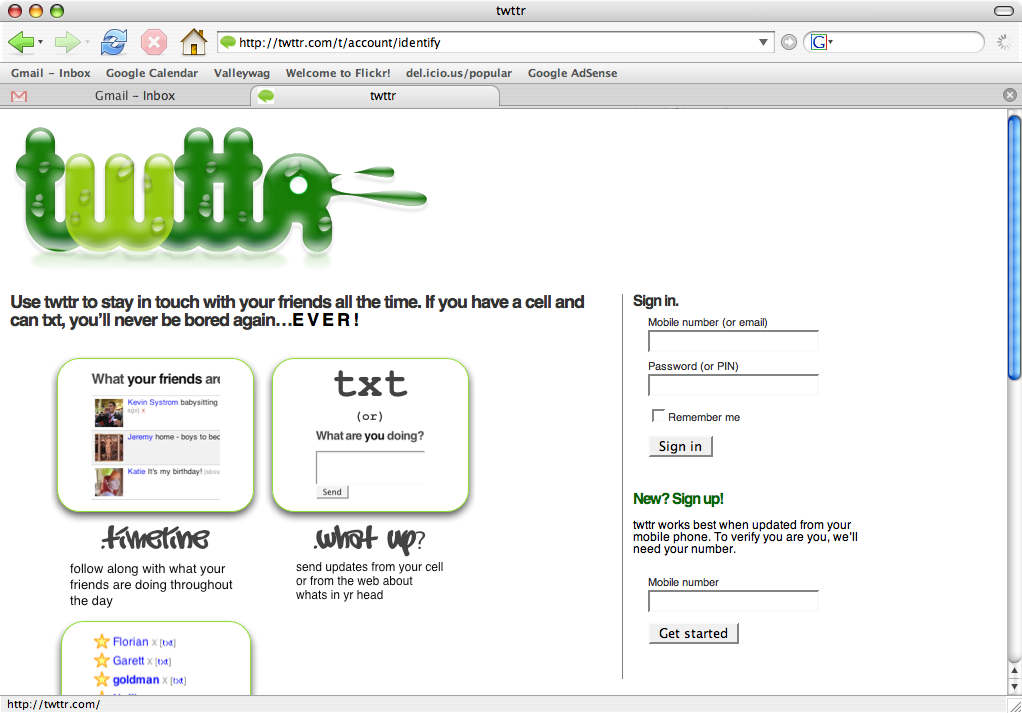
\includegraphics[width=1.0\textwidth, height=125px]{Images/Design/Twitter_2006}
		\caption{Twitter in 2006}\label{fig:Twitter_2006}		
	\end{subfigure}
	\quad
	\begin{subfigure}[t]{0.45\textwidth}
		\centering
		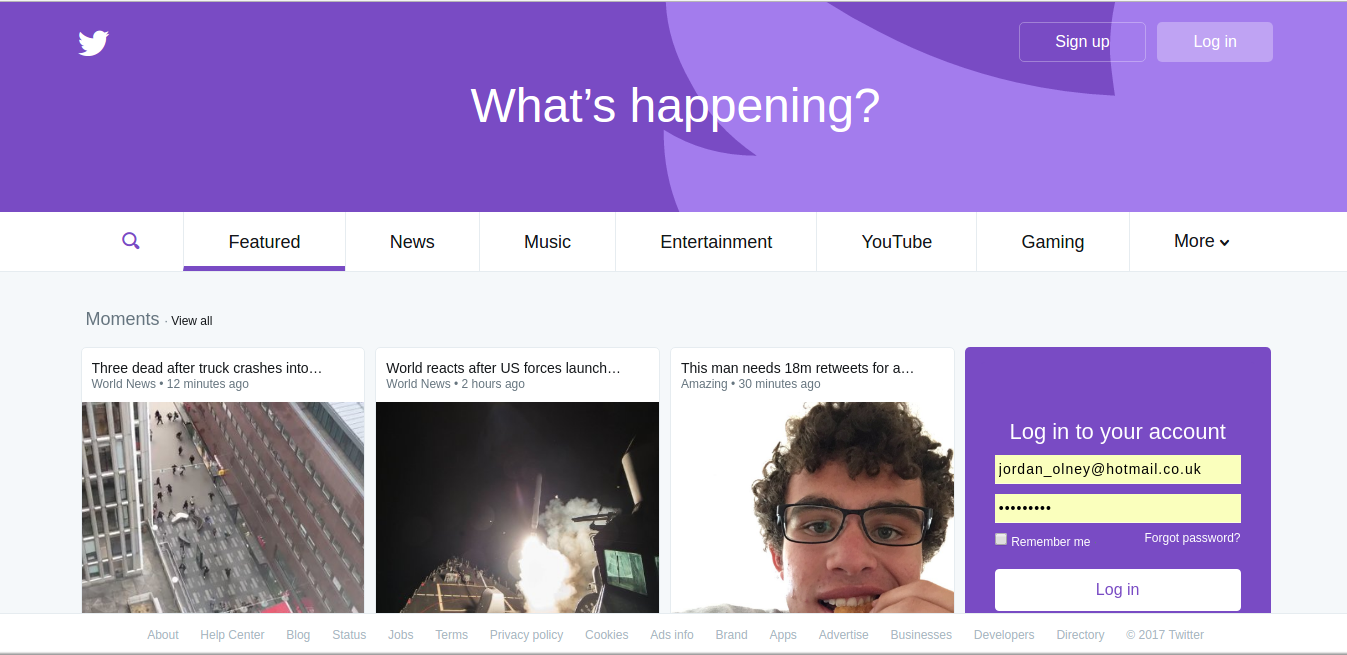
\includegraphics[width=1.0\textwidth, height=125px]{Images/Design/Twitter_2017}
		\caption{Twitter in 2017}\label{fig:Twitter_2017}
	\end{subfigure}
	\caption{Twitter in 2006 and 2017}\label{fig:Twitter_Changes}
\end{figure}

\subsection{Consistency}
By ensuring that the design of the application is consistent across all pages in the site, users will be able to learn quickly how to navigate and use features of the site. An example of this is the navigation bar, which will be included on all of the pages, allowing the user to search and log in and out. Figure \ref{fig:navs} demonstrates how Facebook and Twitter have designed a similar navigation bar which features throughout their site. Also, Fidelis will make use of widgets, which can be reproduced on multiple pages across the site. This allows features to be repeated, without having to change style. Doing so allows the users to understand the possible actions they are able to make on each page and improves ease of use.

\subsection{Familiarity}
Whilst aiming to differentiate Fidelis from other social networks by implementing features which make it more trust-centric, keeping a familiar design will allow users to use the site with minimum learning. Therefore, language used on the site will be similar to the language in pre-existing social networks. This includes the terms `following' and `followers' to describe who a user is connected to within the network and `trending' to show the most common terms which are being mentioned within a period of time. In addition, the hash symbol will be used to tag a post and @ will be use to mention a user in a post, as is the case with social networks such as Twitter, Instagram and Facebook. Other features such as profile picture, wallpapers and notifications will also follow a familiar format in comparison with current popular websites.

\subsection{Intuitive Design}
By using an intuitive design, the usability of Fidelis will increase, as it would become easier and quicker for users to complete tasks. For example, affordances could be used so that the purpose of a feature becomes obvious to the user through the design only. This could include using a magnifying glass to symbolise search or using a dust bin for deleting an item. There is also additional functionality which can be added to the site to make navigation more intuitive, such as clicking on the logo to redirect to the home page. Furthermore, displaying search suggestions as a user types in the search bar allows the user to quickly navigate to the desired page without having to redirect to a search results page. Not only this, but showing search suggestions aids ease of use, such as when the user is unsure of spelling. Figure \ref{fig:fb-search} shows how Facebook have designed their search alongside suggestions.

\begin{figure}[H]
	\centering
	
\includegraphics[height=125px]{Images/Design/fb-search}
	\caption{Facebook search}\label{fig:fb-search}		
\end{figure}
\section{User Interface}
The user interface (UI) is perhaps one of the most important aspects of Fidelis; the UI dictates how users interact with the system, and serves as the single point of entry for user data. Fidelis needs to be able to engage the audience from the moment they land on the homepage and encourage the users to explore further by providing an easy to use and intuitive UI. This can be achieved by following standards defined by several committees and adhering to good practices. In addition to the engagement the Fidelis UI must also be usable and simple whilst remaining elegant and intuitive. Responsive design is also crucial to provide access to the system across a range of devices, and this is discussed later in more detail. The provided designs were produced as mock-ups, but were designed in such a way as to closely replicate the final product.

\subsection{Sitemap}
Figure \ref{fig:sitemap} shows the sitemap for Fidelis. This signifies the navigation routes the user will be able to follow on the site. Both sets of users (authorised and authorised) will be able to visit:
\begin{itemize}
\item Landing page - Users will arrive onto this page when they visit Fidelis for the first time
\item Registration page - This page will allow new users to register an account
\item Log-in page - This page will allow users who already made an account to log-in 
\item Password Recovery page - This page will allow users to reset their password if they have forgotten their account credentials
\item Discover page - The Discover page display posts to users that are sorted into different categories
\item Profile page - The Profile page will include details on a specific user, including the number of posts they have made and the posts they have voted on
\item Privacy page - The Privacy page will provide details on the Fidelis privacy policy
\item Support page - The Support page will provide general support to users, such as Frequency Asked Questions (FAQs)
\end{itemize}

However, the Home page, which will contain a feed of posts from the authorised users and other users the follow, and the Settings page will only be accessible to authorised users.

\begin{figure}[H]
\centering
\includegraphics[height=2.7in]{Images/Design/sitemap}
\caption{Fidelis Sitemap}
\label{fig:sitemap}
\end{figure}

\subsection{Navigation}
A navigation bar provides users with a quick way of accessing pages on a website. The navigation bar is usually located at the top of the page, and includes `quick-link' icons that allow users to easily navigate to pages represented by each icon. Figure \ref{fig:navs} shows the navigation bars for Facebook and Twitter. In both we can see shared elements, such as the profile and home icons. In addition to the icons, the navigation bars also have search boxes. These search boxes enable users to explore content available on each site by providing keywords.

\begin{figure}[H]
\centering
\begin{subfigure}{1\linewidth}
	
\includegraphics[width=1\linewidth]{Images/Design/fb-nav}
	\caption{}
	\label{fig:fb-nav}
\end{subfigure}
\begin{subfigure}{1\linewidth}
	
\includegraphics[width=1\linewidth]{Images/Design/twitter-nav}
	\caption{}
	\label{fig:twitter-nav}
\end{subfigure}
\caption{Navigation bar designs for (a) Facebook and (b) Twitter}
\label{fig:navs}
\end{figure}

By studying existing navigation bar designs, concept designs for navigation on Fidelis were created. These designs can be seen in figure \ref{fig:fidelis-navs}. There will be two navigation bars - one for unauthorised users and the other for authorised users. Both designs employ intuitive icons that will allow the user to identify the page they will be taken to when the icon is clicked on. To signify the page users are currently on, an orange underline will highlight the icon corresponding to the page the user has navigated to. In addition to this, the navigation bar will also include a search field which will allow the user to locate specific categories or users. The two navigation bars differ slightly in the pages they allow the user to navigate to. When a user is not logged in, they will be unable to view their notifications (signified by the bell icon), or view their profile. However, they will still be able to view public posts in a category they search for, or view a public user profile and access the discover page.

\begin{figure}[H]
\centering
\begin{subfigure}{1\linewidth}
	
\includegraphics[width=1\linewidth]{Images/Design/nav-unauthorised}
	\caption{}
	\label{fig:nav-unauth}
\end{subfigure}
\begin{subfigure}{1\linewidth}
	
\includegraphics[width=1\linewidth]{Images/Design/nav-authorised}
	\caption{}
	\label{fig:nav-auth}
\end{subfigure}
\caption{Fidelis navigation bar designs for (a) unauthorised and (b) authorised users}
\label{fig:fidelis-navs}
\end{figure}

\subsection{Authentication}
User authentication involves either collecting the credentials of a user to verify their identity and retrieve the relevant data for that user, or allowing a user to register a new account. These two processes for authentication are normally represented with log-in and registration pages. The following sections will look at the design for each of these.

\subsubsection{Register}
The registration page should enable new users to enter their details and create an account on Fidelis. Sites vary in the details they collect during registration. Figure \ref{fig:reg-pages} shows the registration pages for Twitter and Reddit. Each of the sites collects user email addresses and passwords. These two pieces of information are consistent across almost all registration pages, regardless of the website. In addition to this, Reddit, as seen in figure \ref{fig:reddit-reg} asks only for a username. Twitter registration (figure \ref{fig:twitter-reg}) does not require a username, and instead collect the users full name. Facebook, whose registration is not shown, collects even more user data than both of the aforementioned sites, requiring a date of birth and gender in addition to what is already collected by Twitter. 

\begin{figure}[H]
\centering
\begin{subfigure}[b]{.4\linewidth}
	
\includegraphics[height=1.5in]{Images/Design/twitter-reg}
	\caption{}
	\label{fig:twitter-reg}
\end{subfigure}
\begin{subfigure}[b]{.5\linewidth}
	\centering
	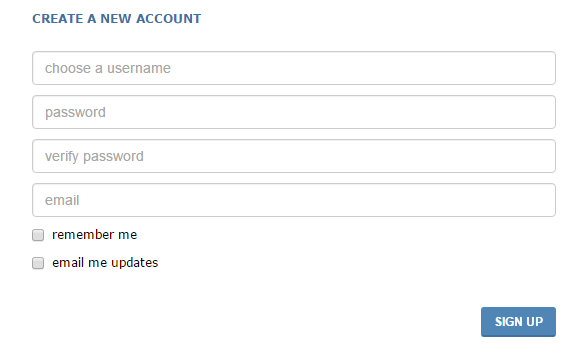
\includegraphics[height=1.5in]{Images/Design/reddit-reg}
	\caption{}
	\label{fig:reddit-reg}
\end{subfigure}
\caption{Registration pages for (a) Twitter and (b) Reddit}
\label{fig:reg-pages}
\end{figure}

Figure \ref{fig:register-page} shows the design for the Fidelis registration page. Users will be required to enter their name, email, username, date of birth and password. Although not entirely necessary initially, it was decided to retain user date of births as thought was put into future uses for it. As the system grows, it is inevitable that certain categories or tags will contain content unsuitable for younger audiences. Therefore, age can be used a tool to filter unsuitable content for younger users. In order to ensure that the users are compliant with the terms of the site, they will be required to to agree to these terms before registration can be completed.

\begin{figure}[H]
\centering
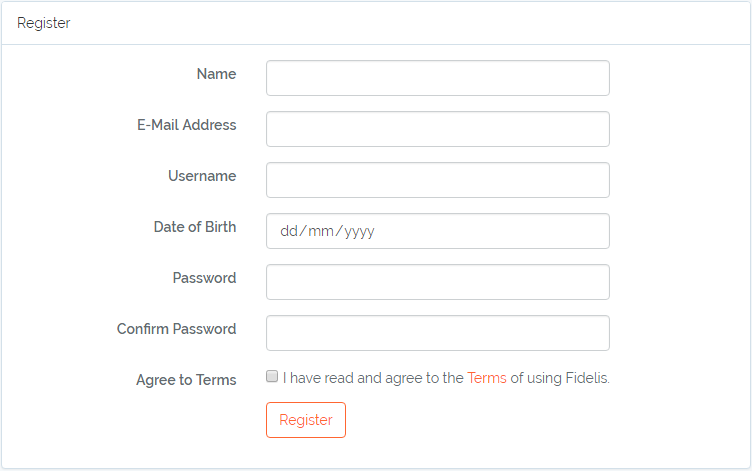
\includegraphics[height=2in]{Images/Design/register-page}
\caption{Design for registration page}
\label{fig:register-page}
\end{figure}

\subsubsection{Log In}
The log-in page should allow an existing user to enter their log-in credentials. On most sites this is a combination of either email or user name, and a password. To be able to correctly verify user identity, both email (or username) and password must be required fields. Users are responsible for remembering their log-in credentials, but are also liable to forget them. To prevent user accounts from being inaccessible, the log-in page should include a link that allows users to recover a forgotten password. A user may accidentally navigate to the log-in page, when they actually intended to navigate to the registration. As such, a link must exist on the log-in page which will take users to the registration page. Figure \ref{fig:login-page} shows the concept design for the log-in page, encapsulating all aforementioned aspects.

\begin{figure}[H]
\centering
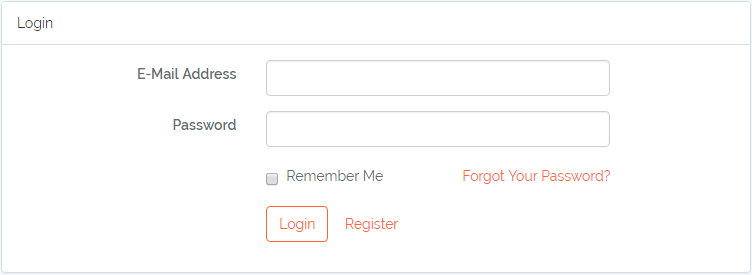
\includegraphics[height=1.5in]{Images/Design/login-page}
\caption{Design for log-in page}
\label{fig:login-page}
\end{figure}

\subsection{Home}
As with most websites, the home page serves as the sites' central hub. This is often the first page that a user will see upon entering the website. Fidelis is no different in this regard. The Fidelis home page is split into two different pages, one for when the user is logged in, another for when they aren't.

\subsubsection{Landing Page}
If a user is not logged onto the website, they will see the page shown in figure \ref{fig:home_unauthorised}. This is the landing page for the site and will be the first port of call for any logged out users or users who are new to Fidelis. The background for this page is a full-screen image, randomly chosen from a select set of images. In the centre of the page there is the title Fidelis, as well as a quote relating to the core concept of the platform - trust. Again, these quotes are chosen randomly from a set of quotes. The user will be able to navigate to either the log-in or registration page using the buttons in the top right of the page.

\begin{figure}[H]
\centering

\includegraphics[width=\linewidth]{Images/Design/home_unauthorised}
\caption{Design for home page when not logged in}
\label{fig:home_unauthorised}
\end{figure}

\subsubsection{Home Page}
Once a user has logged in to their account or registered a new one, they will be directed to the home page, shown in figure \ref{fig:home_authorised}. The page will feature a navigation bar so the user can navigate to other pages, search for tags and users. The most prominent feature of this page is the central post feed. A user will be able to create new posts including text and images as well as being able to interact with other posts. This includes up-voting or down-voting a post, commenting on a post and reporting posts. Users will also have the option to delete posts they have made. The posts displayed in this feed will be selected by the system to match the users' interests.

When creating a post, a tagging system will be used, similar to Twitter, which will allow users to mention other users (using the @ symbol) and also to tag topics (using the \# symbol). These tag topics will be used to create specific topic feeds in the discover page and to calculate the trending topics. Any topic tags which exist in a post will be added to the post-tags table. In addition to tags allocated to a post using the \# symbol, tags will also be added to a post if the post contains a word which already exists in the tags table. This will allow for content which hasn't been explicitly tagged to be available on the discover page.

Other than the post feed the home page design shows a number of widgets the user will be able to interact with. The user profile widget on the left shows information about the user. This widget will link to the users' profile page, and include some relevant information to the user, such as the number of followers they have. Also on the left of the page design is a widget displaying suggestions for other accounts that the user can follow to expand their network. These suggestions will be bespoke for the current user. On the right side of the page is a widget that will show the tags that are currently trending across the entire platform. This is another way that the user can find new content rather than seeing just the posts in their feed.

\begin{figure}[H]
\centering
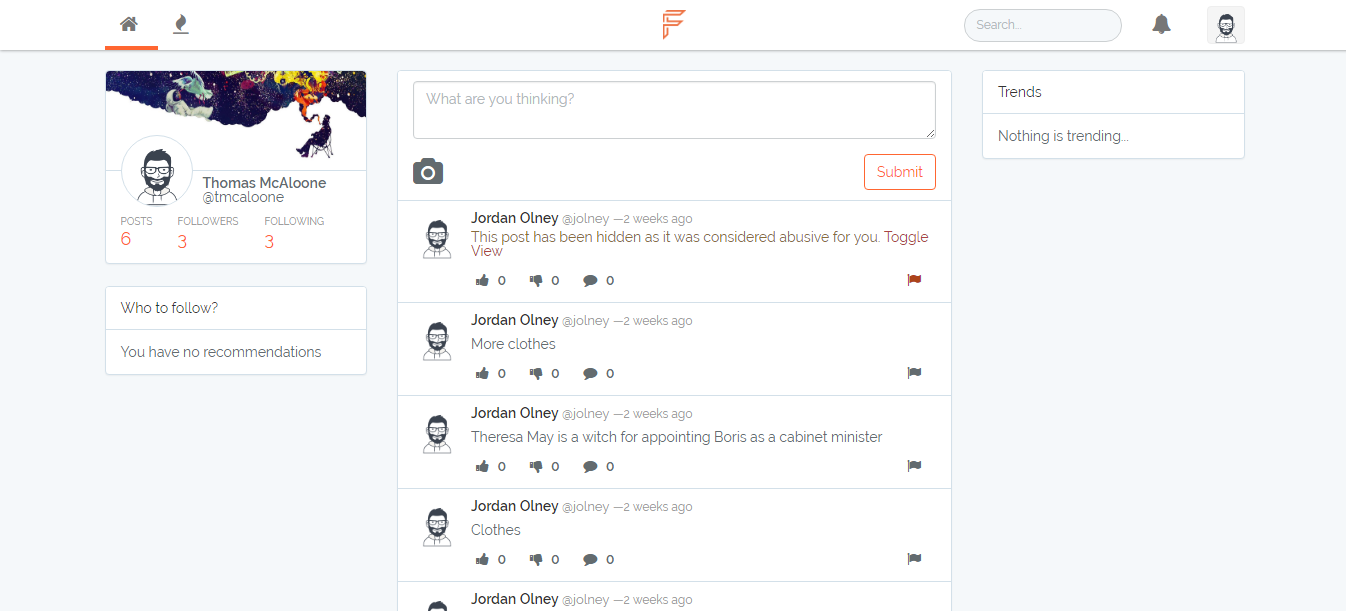
\includegraphics[width=\linewidth]{Images/Design/home_authorised}
\caption{Design for home page when logged in}
\label{fig:home_authorised}
\end{figure}

\subsection{Discover}
A major feature of the Fidelis design is allowing users to seek out and find new content, which appeals to them, outside of their current network. The discover page will allow this to happen. The design for this page, seen in figure \ref{fig:discover_page}, shows a broad list of categories each of which will have a number of tagged posts associated with them that the user can view and interact with.

\begin{figure}[H]
\centering
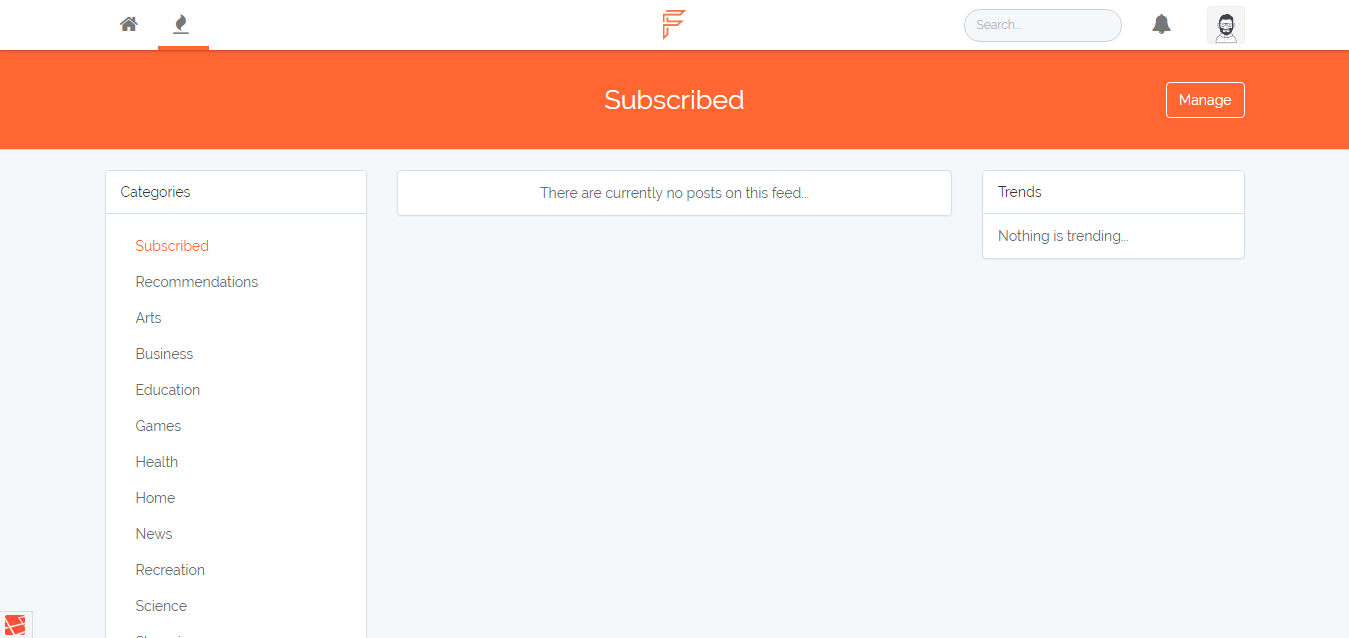
\includegraphics[width=\linewidth]{Images/Design/discover}
\caption{Design for discover page}
\label{fig:discover_page}
\end{figure}

The panel on the left of the page is the category list widget, displaying the categories that will be used to group posts. The user will be able to select a category to see posts that fit with that category. Alternatively, the user can use the widget on the right of the page named `For You'. This will allow the user to select `Subscribed' to see content matching the tags a user is subscribed to, or `Recommended' to view content recommended to them. This list also shows a `Subscribed' option, which when selected will show posts from topics the user is subscribed to. When a category is selected, the title of that category will appear as a title across the top of the page. In the case of the `Subscribed' option, a `Manage' button will also be shown here which will link to the Settings page, where the user can manage (add or remove) their subscriptions. In the centre of the page is the post feed, which in a similar manner to the post feed in the home page design, will show a list of posts the user can interact with, however in this case the posts shown will only be those that belong to the currently selected category. On the right hand of the page is the trends widget which will show all of the tags which are currently trending across the entire Fidelis platform.

\subsection{Notifications}
Notifications are a key component to communication on social media platforms. Notifications give prompts to users on interactions that have occurred between them and other users. To let users know of a new interaction, notifications either give visual or auditory triggers that get a users attention. With the Google Chrome Notifiations API \cite{ChromeAPI:Notifications} it is now even possible to send notifications to users when they are not on the webpage itself. However, notifications on Fidelis will be provided using a number counter next to a bell icon, which will symbolise the notifications page. This is akin to the notification counter seen on most social media platforms. The page itself will contain a feed of notifications that will give information to the user on who the notification is from, and the type of notification it is. If the notification is a comment, it will include the comment from the user making it. If the notification is for a vote or a follow, it will only include information on the name of the user making the vote or follow. Figure \ref{fig:notifications-page} shows a mock-up of how the notifications page will appear. Here we can see a number counter next to the bell icon signifying the number of new notifications, and also a notification telling us that another user has commented on one of the posts we have made. In addition to the notifications themselves, the page will also include profile, recommendations and trending widgets. The user will be able to navigate to their profile from this page, and also interact with trending topics or new user recommendations.

\begin{figure}[H]
\centering
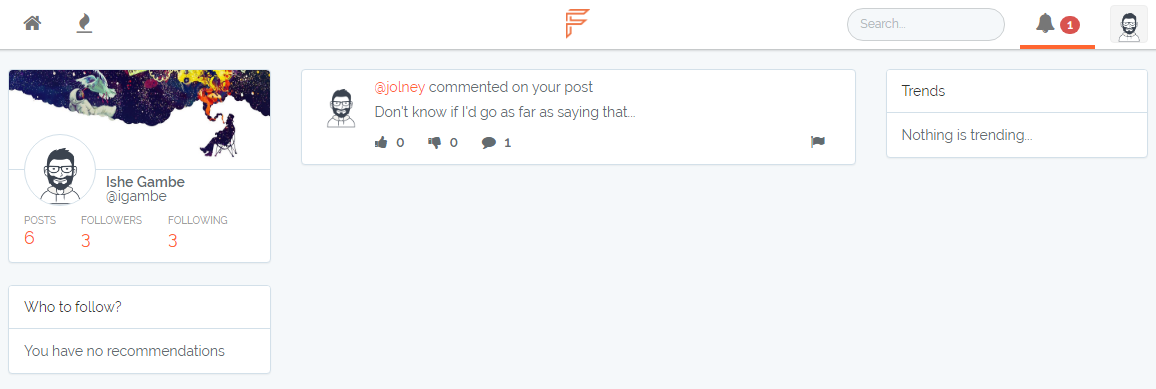
\includegraphics[width=1\linewidth]{Images/Design/notifications-page}
\caption{Design for Notifications page}
\label{fig:notifications-page}
\end{figure}

\subsection{Profile}
The user profile page (shown in figure \ref{fig:user_profile}) is designed to allow the user to see all of their activity and public information related to their account (Name, bio etc.). Here there will also be a display of the user's reputation to give an immediate indication of trustworthiness for this user and their content. The user will also be able to view the profiles of other users, creating yet another avenue for discovering new content, as well as nurturing user-to-user interactions across the platform. Along the top of the page one can see the users' profile photo and cover photo, a feature which will allow a user some expression to aid in building a user's personal presence on the platform. If the current page belongs to the user viewing it, the user will be able to change their profile or cover photo by clicking and icon that will appear when the cursor hovers over either image. Below the user's profile we can see some personal information related to the user. Here we also see a widget of photos that the user has uploaded. In the centre of the page we see a post feed which will display content the user can interact with. The content displayed will be based upon which tab the user currently has selected. These tabs can be seen directly above the post feed. The posts tab will display all of the posts created by the user to whom the page belongs. The rated tab will display a history of all the posts that the user has rated (up-voted or down-voted). The follower and following tabs will display a list of all of the other users that this user follows, or is followed by respectively. The trending widget on the right of the page will show all of the tags currently trending across the platform. Finally there is a button on the right side of the page which changes depending on to whom the page belongs. If the current page is being viewed by its owner, the user will be given a prompt to edit their profile, in case there is any information they want to add, update or remove. If the profile page being viewed is owned by someone who is not the user, the user will be given the opportunity to follow, unfollow or block the user who owns this page.

\begin{figure}[H]
\centering
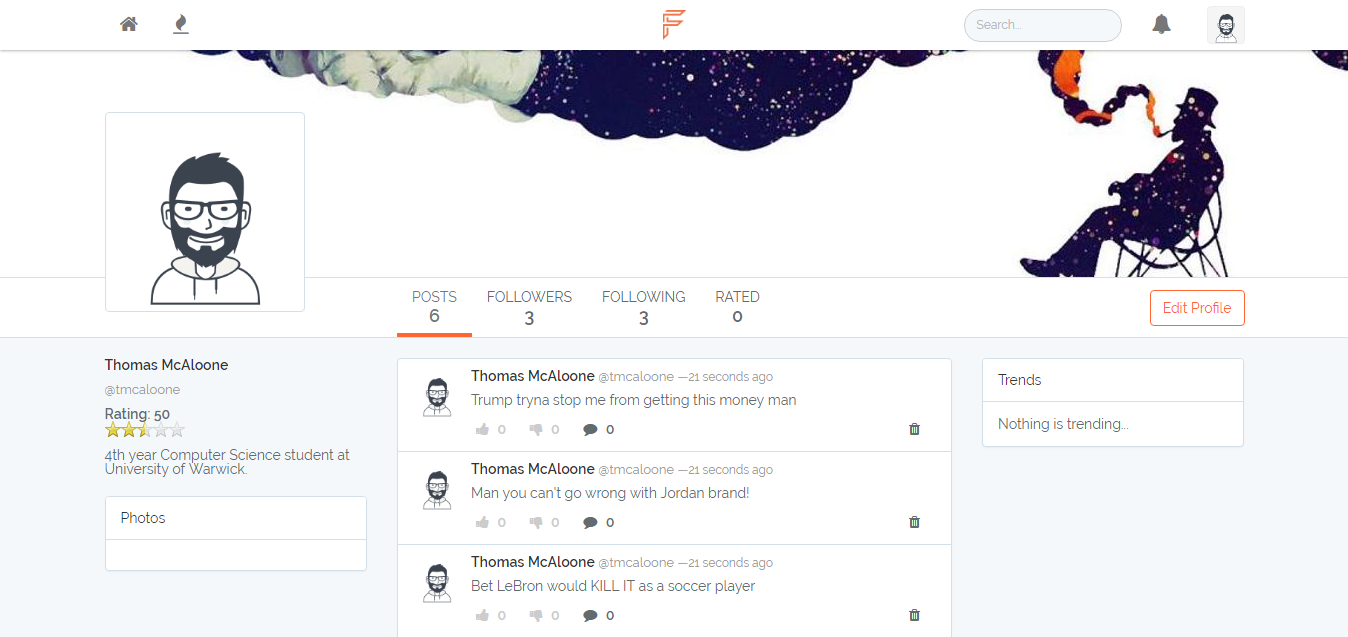
\includegraphics[width=\linewidth]{Images/Design/user_profile}
\caption{Design for user profile page}
\label{fig:user_profile}
\end{figure}

\subsection{Settings}
The settings page will enable users to make changes to their user profile. It is important to provide users with the option to monitor and change their profile settings as they see fit. This gives them control over their account. Settings generally included for user accounts include the ability to change their email address or update their passwords. Some websites, like Facebook and Google, allow users to control devices linked to the user account.

\begin{figure}[H]
\centering
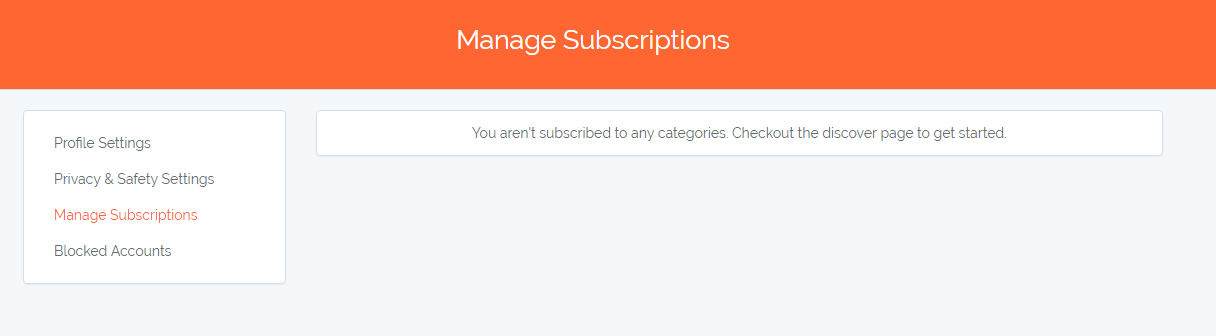
\includegraphics[height=1.5in]{Images/Design/SettingsPage}
\caption{Design for user settings page}
\label{fig:SettingsPage}
\end{figure}

Figure \ref{fig:SettingsPage} shows the design for the user settings page. Settings will be divided into: profile settings, privacy \& safety settings, tag subscription management and managing blocked accounts. Profile settings will allow the user to change their name or username, and toggle the privacy of their account. Privacy \& safety settings will provide users with a set of parameters used for data processing. The parameter values chosen by users will determine the outcome of data processing. An example parameter under the safety settings will be the reputation threshold that will be used during recommendation generation. The subscription management tab will allow users to view tags they are subscribed to, and unsubscribe from them if they no longer wish to see their content. Finally, the blocked accounts tab will enable the user to view users they have blocked, and will provide the user with the option to unblock previously blocked users.

\subsection{Static Pages}
The two static pages aim to address the possible issues discussed in section \ref{Chapter:Issues}, by displaying information about the terms of use for Fidelis and providing support in order to help alleviate any personal issues which can arise through the use of social networking sites. These pages are accessible to both authorised users and guests visiting Fidelis. Both static pages are accessible via links in the footer of every page.

\subsubsection{Support}
The support page displays details of how to deal with content on the site which may distress the user. Fidelis aims to keep this content to a minimum, through abuse detection, reputation scoring and terms of service. However, some content may still be posted on the platform which is not prevented via these measures. Therefore, the page lists options of how to remove the content: by reporting it and adjusting abuse detection settings. It also provides contact details to the Samaritans \cite{Samaritans:Home}, who can offer support in case of any social issues which may arise on the network such as cyber-bullying. As seen in figure \ref{fig:support}, the styling for the page is simplistic, using bullet points in order to break down the information being provided.

\begin{figure}[H]
\centering
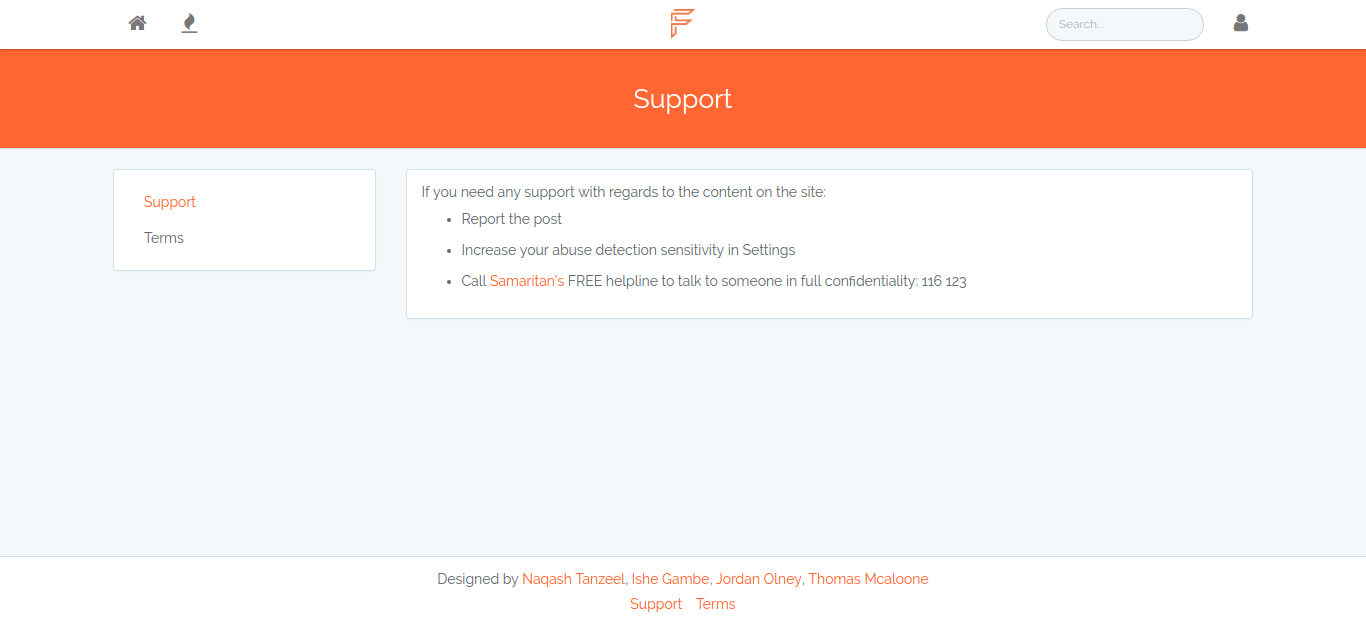
\includegraphics[height=2in]{Images/Design/support-page}
\caption{Design for support page}
\label{fig:support}
\end{figure}

\subsubsection{Terms}
The styling for the terms page is the same as the support page, using bullet points to make the information more readable, as shown in figure \ref{fig:terms}. However, the information provided is regarding the terms of service, to ensure that the user understands what is expected of them when using the site and the service Fidelis is expected to provide. This is to help avoid any legal issues which may arise from the content which is posted on the site by users.

\begin{figure}[H]
\centering
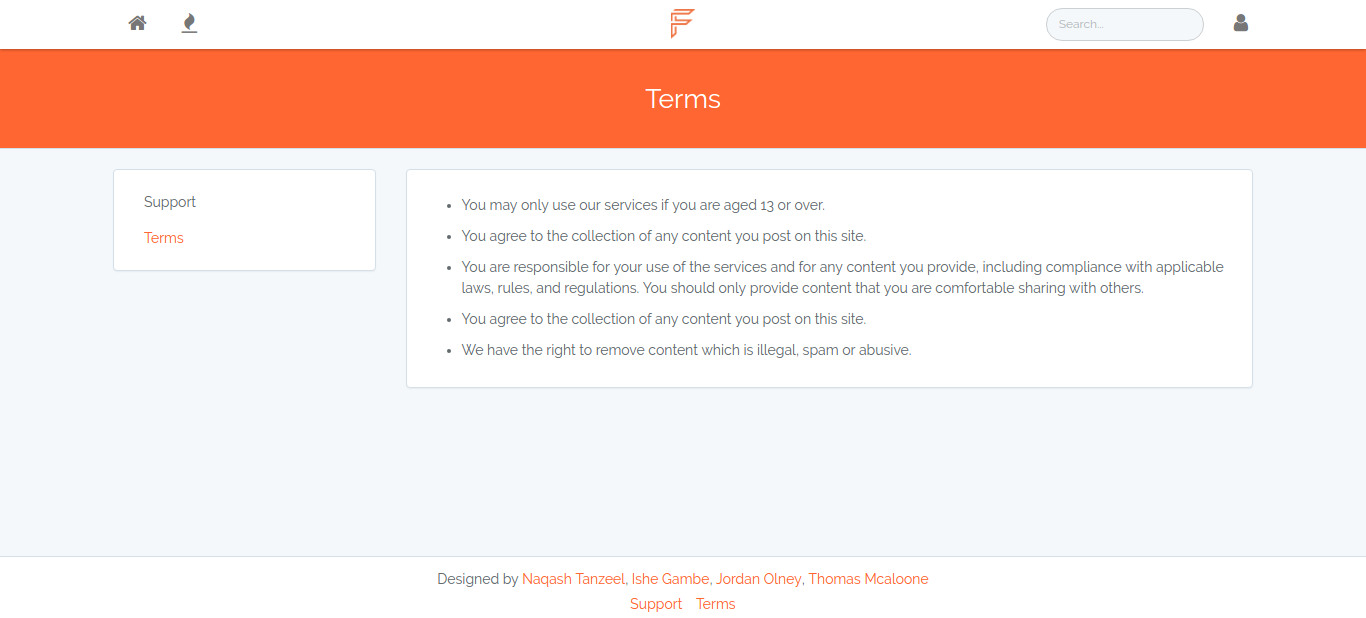
\includegraphics[height=2in]{Images/Design/terms-page}
\caption{Design for terms page}
\label{fig:terms}
\end{figure}

\subsection{Widgets}
Widgets are re-usable ``miniature application views'' that provide specified, limited functionality \cite{AndroidDevelopers:Widgets}. Widgets are extremely popular on mobile devices; in figure \ref{fig:WeatherWidget} we can see a widget for the weather. 

\begin{figure}[H]
\centering

\includegraphics[height=1in]{Images/Design/AppWidget}
\caption{Weather widget from an Android phone}
\label{fig:WeatherWidget}
\end{figure}

Widgets are a convenient way of modularising key application functionalities that can be repeated across multiple web pages. Because of this, widgets will be used on Fidelis to relay information to the user in a consistent manner. Namely, these widgets are:

\begin{itemize}
\item The profile widget, which will provide a summary of key user information, such as the number of posts they have made
\item The trending widget, which will provide the user with a list of up-to-date trending topics
\item The recommendations widget, which will display custom user recommendations to the user
\end{itemize}

This section will discuss the design of each of these widgets in more detail.

\subsubsection{Profile}
The profile widget is responsible for displaying basic profile information for a user. The widget was designed in the form a of a profile card. It shows the users' cover photo at the top along with their profile photo, much like the actual profile page. Additionally, basic information like name and username along with number of posts, followers, and following is also displayed. When displaying another users profile, interactive relationship toggles are also provided. The design is consistent across the two different versions of the widget and can be seen in \ref{fig:ProfileWidget}.

\begin{figure}[H]
	\centering
	\begin{subfigure}[b]{0.5\linewidth}
		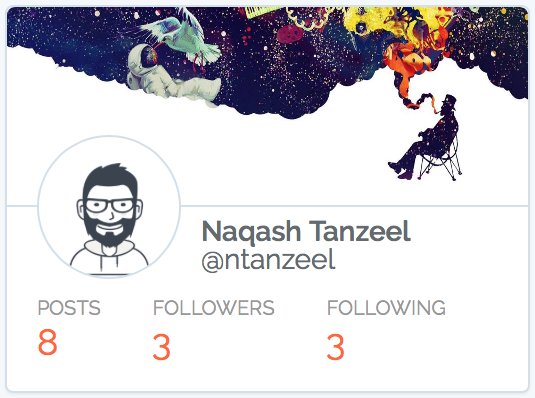
\includegraphics[width=1\textwidth]{Images/Design/UI/Widgets/Profile_Self}
		\caption{Self Profile}
		\label{fig:ProfileWidget_Self}
	\end{subfigure}
	\begin{subfigure}[b]{0.4\linewidth}
		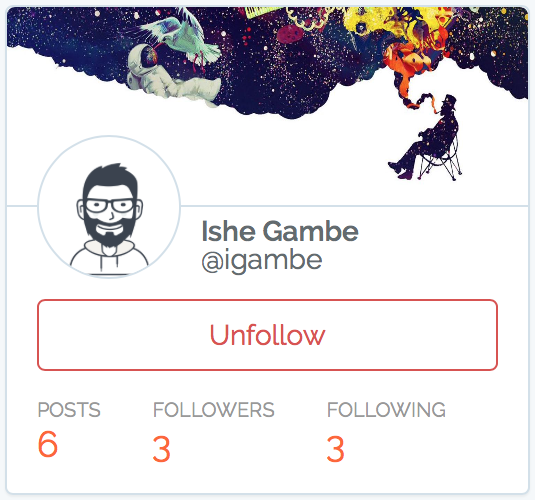
\includegraphics[width=1\textwidth]{Images/Design/UI/Widgets/Profile_Other}
		\caption{Others Profile}
		\label{fig:ProfileWidget_Other}
	\end{subfigure}
	\caption{The profile widget when displaying your own and someone else's profile}
	\label{fig:ProfileWidget}
\end{figure}


\subsubsection{Trending} \label{sec:design-trending}
The widget shown in figure \ref{fig:trending} displays the top trending tags. The tags are displayed in descending order of how common they were in the last half an hour. Each trending tag is a link to the corresponding tags' feed on the discover page, allowing the user to find content relevant to that tag. The design of the widget is similar to the trending widget found on Twitter (see figure \ref{fig:trending-twitter}), so that the user is familiar with the functionality it provides.

\begin{figure}[H]
	\centering
	\begin{subfigure}[b]{0.4\linewidth}
		
\includegraphics[width=1\textwidth]{Images/Design/trending-widget}
		\caption{Trending on Fidelis}
		\label{fig:trending}
	\end{subfigure}
	\begin{subfigure}[b]{0.4\linewidth}
		
\includegraphics[width=1\textwidth]{Images/Design/trending-twitter}
		\caption{Trending on Twitter}
		\label{fig:trending-twitter}
	\end{subfigure}
	\caption{Trending widgets on Fidelis and Twitter}
	\label{fig:TrendingWidgets}
\end{figure}

\subsubsection{Recommendations}
User recommendations that will be generated as discussed earlier in section \ref{sec:ContentRecommendation} will need to be displayed to the user. Figure \ref{fig:RecommendationsWidgetDesign} shows the design for the user recommendations widget. The widget will show the user any new recommendations that have been generated for them, or old recommendations they have not interacted with. The widget will allow users to navigate to the profile of the recommendation, and will also have buttons which will enable the user to accept or reject the recommendations they have been provided with.

\begin{figure}[H]
\centering

\includegraphics[height=1.5in]{Images/Design/RecommendationsWidgetDesign}
\caption{Design for the recommendations widget}
\label{fig:RecommendationsWidgetDesign}
\end{figure}

By providing recommendations as a widget, this will allow recommendations to be displayed to the user on multiple pages. With this in mind, the recommendations widget will appear for authorised users on the home, notifications and profile page.

\section{Responsive Design}
Mobile phones and handheld devices are reshaping how we view technology. Their portable nature and accessibility have meant that a growing number of the worlds popultion own a mobile phone. In 2017, a predicted 4.77 billion people worldwide own a mobile phone \cite{Statista:Mobile}. This is more than half of the global population. An even more staggering statistic is that roughly half of the mobile phones owned are smartphones \cite{Statista:Smartphones}. Smartphones have broadened the scope of internet availability through the advanced capabilities most modern smartphones come equipped with. In fact, for the first ever in 2016 internet traffic from mobile phones and tablets exceeded that of desktops, accounting for 51.3\% of internet usage \cite{StatCounter:MobileInternetTraffic}. Taking all of this into consideration, it would make no sense to design a web application only fit for purpose on desktops; there must be thought put into building a web application suitable for any and all devices. To this end, Fidelis must be easily usable regardless of the device it is being viewed on, as long as a modern browser is used. For smaller devices, navigation will be hidden to make more room for content on the page. In addition to this, content will be resized based on the size of the screen so that it is clearer and can be read easily without having to pan in and out.

\begin{figure}[h]
	\centering
	\begin{subfigure}[b]{.45\linewidth}
		
\includegraphics[height=2.5in]{Images/Design/FidelisMobile}
		\caption{}
		\label{fig:mobile-responsive}
	\end{subfigure}
	\begin{subfigure}[b]{.45\linewidth}
		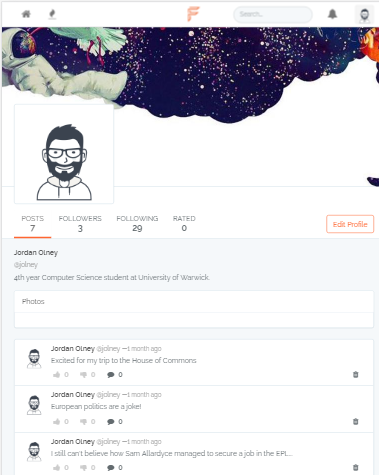
\includegraphics[height=3in]{Images/Design/FidelisIpad}
		\caption{}
		\label{fig:ipad-responsive}
	\end{subfigure}
	\caption{The Fidelis profile page as it appears on (a) Mobile phones and (b) Handheld devices}
	\label{fig:responsive}
\end{figure}

Consideration of mobile and handheld devices will strongly influence the design decisions made as certain features will be achievable on devices with lower resolutions whereas other features will make pages appear empty on larger resolution devices. Figure \ref{fig:responsive} shows the profile page as it will appear on handheld devices of varying sizes. In both designs, we see some features are hidden. For example, on the mobile device in Figure \ref{fig:mobile-responsive}, the navigation bar is condensed into a menu button which the user can touch to reveal the same options available normally. 